\documentclass[12pt, letterpaper, twoside]{article}
\usepackage[utf8]{inputenc}

\usepackage{geometry}
\usepackage{algorithm}
\usepackage{algpseudocode}
\usepackage[backend=bibtex,style=verbose-trad2]{biblatex}
\usepackage{amssymb}
\usepackage{amsmath}

\setlength{\parindent}{4em}
\setlength{\parskip}{1em}
\bibliography{citation-13218946}

\title{Solucionando el problema de la mochila en el Modelo Sticker}
\author{Ernesto Mancebo}
\date{Febrero 2020}

% \tikzset{
%     pics/realline/.style 2 args = {
%         code = {
%             \draw [thick] (0,0) -- (6,0) node [right=2mm] {$$mathbb{R}};
%             \fill[black] (1,0) circle (1mm) node[abobe=2mm] {$#1$}
%                          (3,0) circle (1mm) node[abobe=2mm] {$#2$}
%                          (6,0) circle (1mm) node[abobe=2mm] {$V_4$};
%             \foreach \i [count=\j] in {0,0.5,1,1.5,3,4.5,6}
%                 \coordinate (-\j) at (i,0);
%         }
%     }
% }
\usepackage{tikz}
%\usetikzlibrary{positioning}

\tikzset{
  mynode/.style={fill,circle,inner sep=2pt,outer sep=0pt}
}


\begin{document}
    \maketitle
    \begin{abstract}
        Este documento ***
    \end{abstract}

    \section{Introducción}
    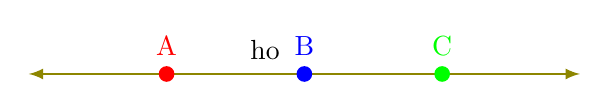
\begin{tikzpicture}
        \draw[olive,thick,latex-latex] (0,0) -- (7,0)
        node[pos=0.25,mynode,fill=red,label=above:\textcolor{red}{A}]{}
        node[pos=0.5,mynode,fill=blue,text=blue,label=above:\textcolor{blue}{B}]{}
        node[pos=0.75,mynode,fill=green,text=green,label=above:\textcolor{green}{C}]{};

        \node at (3,0.3) {ho};
      \end{tikzpicture}

    \section{Modelo Sticker}
    \par El Modelo Sticker es un modelo de computación inpirado en cadenas de ADN propuesto por Sam Roweis \cite{citation-13218946}, donde tal modelo se basa en procedimientos de filtrado y con memoria de acceso aleatorio. En ese mismo orden, se distingue de otros modelos computacionales por la manera en que representa la información.

    \subsection{Conceptop de Cadena de Memoria}

    \par El eje central de este modelo son las cadenas de memoria, tales cadenas consisten en hebras simples de ADN configuradas de forma $(n, k, m)$, tal que $n\geq k.m$, siendo $n$ la cantidad de sub-cadenas que soportra, $k$ las sub-cadenas dentro de $n$, y $m$ la longitud de cada sub-cadena $p$. Las cadenas de memoria también se les conocen como moléculas y son representadas por sigma ($\sigma$).
    \par En ese orden, las operaciones realizadas sobre cada hebra o complejo de memoria asocia un sticker a una región $k$, transformando la cadena en una hebra doble \emph{parcial}, tal que en cada región donde haya un sticker complementándole se dice que está \emph{encendido}, mientras que la región donde se carezca de sticker se dice está \emph{apagado}. Tal abstracción binaria también se puede expresar de modo \emph{0/1}.\\



    \subsection{Codificación de la Información}

    \subsection{Concepto de Tubo}
    \par Dentro de este modelo, conocemos un tubo como un multiconjunto de complejos de memorias del mismo tipo. Tal concepto se puede ilustrar del modo:
        $
        \begin{aligned}
            &\begin{bmatrix}
                    & \sigma_0 \\
                    & \sigma_i \\
                    & \sigma_{i + 1} 
                \end{bmatrix}
            \end{aligned}
        $
    \par En ese orden de ideas, las operaciones a principales dentro de este modelo son:
    \begin{itemize}
        \item \emph{mezclar}$(T_1,T_2)$: Retorna la unión de los dos tubos devolviendo un solo tubo el cual contiene cada complejo de memoria proveniente de ambos. También se nota como $(T_1\bigcup T_2)$.
        \item \emph{separar}$(T, i)$: Para un tubo $T$ y un $i$ tal que $(1 \leq i \leq n)$, siendo $n$ la cantidad de subcadenas para cada complejo de memoria, retorna un $+(T, i)$ y $-(T, i)$, de modo que el primer tubo contiene todos los complejos de memoria cuya región $i$ esté encendida (\emph{on} o $1$), mientras que la segunda lo contrario (\emph{off} o $0$).
        \item \emph{encender}$(T, i)$: Para un tubo $T$ y un $i$ tal que $(1 \leq i \leq n)$, siendo $n$ la cantidad de subcadenas para cada complejo de memoria, enciende la región $i$ de cada complejo de memoria asignando un $1$ u \emph{on}.
        \item \emph{apagar}$(T, i)$: Opuesto a \emph{encender}, asigna un $0$ u \emph{off}.
        \item \emph{leer}$(T)$: Dado un tubo $T\neq\emptyset$, lee su contenido.
    \end{itemize}
    \subsection{Concepto de Librería}
    \par Una librería dentro de este modelo es lo conocido como complejos de memoria de modo $(k,l)$ tal que $(1 \leq k \leq l)$, teniendo $k$ sub cadenas/regiones y las primeras $k - l$ subcadenas están \emph{on} u \emph{off}, en todas sus posibles combinaciones.

    \section{Sub-Rutina Ordenado por Cardinalidad}
    \par Teniendo los siguientes elementos:
    \begin{itemize}
        \item $A = \{1,\cdots,p\}$
        \item $B = \{b_1,\cdots,b_s\} \subseteq A$ 
        \item $F = \{D_1,\cdots,D_t\} \subseteq P(A)$ 
    \end{itemize}
    \par Se busca ordenar $F$ con respecto a su cardinalidad en $B$, o en otras palabras, la cantidad de elementos que conincidan de manera $B\cap D_i$.
    \par Una vez teniendo claro el domino del problema planteado, el paper bajo estudio nos sugiere el implementar la codificación de cada familia de subconjuntos $F$, de forma que la familia mencionada sea una molécula $\sigma$ para el tubo $T_0$, codificando cada molécula de forma $T_0=\{\{\sigma:|\sigma|=p \land \exists j(\chi_{D_j}=\sigma)\}\}$; tal que $\chi_{D_j}$ es la función característica en $A$, siendo $(\chi_{D_j}(i) = 1$ si $i \in D_j$ de lo contrario $\chi_{D_j} = 0$ si $i \in A - D_j)$.
    \par Ya con las restrinciones definidas, se plantea en el paper una subrutina que en el paso \emph{i} se generen $i + 1$ tubos verificando la condición $\forall\sigma(\sigma\in T_j \rightarrow|\sigma\in\{b_1,\cdots,b_i\}|=j)$, leyéndose esta condición: sólo existirán moléculas $\sigma$ en $T_j$ cuya cantidad de regiones encendidas sean igual a $j$.
    \subsection{Algoritmo}
    \par En ese sentido, el paper ** sugiere el siguiente algoritmo:
    \begin{algorithm}
        \caption{Ordena los elementos en $T_0$ con respecto a los elementos de $B$ presentes en cada $\sigma$}
        \label{CardinalSort}
        \begin{algorithmic}[1]
            \Procedure{$Cardinal\_Sort$}{$T_0,B$}
            \For { $i=1$ to $s$ }
            \State $(T_0, T'_0) = separar(T_0, b_i)$
            
            \For { $j=0$ to $i-1$ }
            \State {$(T'_{j+1},T''_j) = separar(T_j,b_i)$}
            \State {$T_j=mezclar(T'_j,T''_j)$}
            \EndFor
            \State {$T_i=T'_i$}
            \EndFor
            \State Return $[T_0,...,T_s]$
            \EndProcedure
        \end{algorithmic}
    \end{algorithm}
    
    \subsection{Traza Sub-Rutina Ordenado por Cardinalidad}
    \par A modo de ilustrar el comportamiendo y los conceptos empleados en el algoritmo concebido, tenemos:
    \begin{itemize}
        \item $A: \{0, 1, 2, 3, 4, 5, 6\}$
        \item $B: \{1, 2, 4\}$
        \item $F: \{[2, 6], [3], [4], [2, 4]\}$
    \end{itemize}
    \par Observemos que los elementos que cumplen $B\cap D_j$ en $F$ son: $\{[\textcolor{red}{2}, 6], [3], [\textcolor{red}{4}], [\textcolor{red}{2, 4}]\}$, cuyos elementos resaltados nos sugieren en qué posición del tubo de salida tras ser evaluados por \emph{Cardinal\_Sort}. Codificando $F$ para llevarlo a un tubo tendíamos: \\
    $
        \begin{bmatrix}
            [0, 0, 1, 0, 0, 0, 1] \\
            [0, 0, 0, 1, 0, 0, 0] \\
            [0, 0, 0, 0, 1, 0, 0] \\
            [0, 0, 1, 0, 1, 0, 0] \\
        \end{bmatrix}
    $
    \par Este $T_0$ codificando $F$ tras la ejecución de \emph{Cardinal\_Sort} tendremos: \\
    $
    \begin{bmatrix}
            T_0&: [[0, 0, 0, 1, 0, 0, 0]] \\
            T_1&: [[0, 0, 0, 0, 1, 0, 0], [0, 0, 1, 0, 0, 0, 1]] \\
            T_2&: [[0, 0, 1, 0, 1, 0, 0]] \\
            T_3&: [] \\
            T_4&: [] \\
            T_5&: [] \\
            T_6&: [] 
    \end{bmatrix}
    $
    \par Cumpliendo de esta manera la condición de $\forall\sigma(\sigma\in T_j \rightarrow|\sigma\in\{b_1,\cdots,b_i\}|=j)$.

    \subsection{Asunciones}
    \par Para usos posteriores dentro de este informe, podemos notar la llamada a \emph{Cardinal\_Sort} de modo:
    \begin{itemize}
        \item $Cardinal\_Sort(T_0)$ cuando $B=A$.
        \item $Cardinal\_Sort(T_0, l, k)$ cuando $B=\{l, l+1,\cdots,k\}$.
    \end{itemize}
    \section{Sub-Rutina de Llenado}
    \par Una vez pensado en el concepto de codificar en $F$ las moléculas $\sigma$ tal que $B\cap D_i$, podemos considerar la idea de segmentar cada molécula $\sigma$ en $T_0$ en las regiones:
    \begin{itemize}
        
        
        \item $(A\sigma )=\sigma (1)\cdots\sigma (p)$
        \item $(L\sigma )=\sigma (p+1)\cdots\sigma (p+r)$
        \item $(F\sigma)=\sigma(p+r+1)\cdots\sigma(p+r+q_f)$
        \item $(R\sigma)=\sigma(p+r+q_f+1)\cdots$
    \end{itemize} 
   \par El propósito de esta sub-rutina es manipular el tubo $T_0$ a fin de modificar las moléculas en $(F\sigma)$ y codifiquen su peso con respecto a $f$ en el sub-conjunto $A$, ambos recursos a definir en breve. Con relación a $(L\sigma) \& (R\sigma)$, no se utilizarán en la subrutina bajo estudio, mas nos será útil delimitar estas regiones para casos posteriores.
   \par Los recursos a utilizar en esta subrutina tenemos:\\
   \begin{itemize}
       \item $A=\{1,\cdots,p\}$
       \item $r \in \mathbb{N}$
       \item $f:A\rightarrow\mathbb{N}$
   \end{itemize}
   \par También se ha de tomar en cuenta que si $B\subseteq A$, denotamos $f(B)=\sum_{i\in B}f(i)$. En ese mismo orden, definimos que $q_f=f(A)$, tal que $A_i=\{1,\cdots,i\}$ siendo $(i\leq i\leq p)$, y $T_0$ un multiconjunto de forma $(n,k,m)$ de complejos de memorías $\sigma$ cuyo $k\geq p+r+q_f$.
   \subsection{Algoritmo}
    \begin{algorithm}
        \caption{Asigna valores para cada complejo de memoria $\sigma$ a partir de la región especificada en $p$ y $r$}
        \label{ParallelFill}
        \begin{algorithmic}[1]
            \Procedure{$Parallel\_Fill$}{$T_0,f,p,r$}
            \For { $i=1$ to $p$ }
                \State $(T^+_{i,0}, T^-_i) = separar(T_{i-1}, i)$

                \For { $j=1$ to $f(i)$ }
                    \State {$r_i=p+r+f(A_{i-1})+j$}
                    \State {$T^+_{i,j}=encender(T^+_{i,j},r_i)$}
                \EndFor
                \State {$T_i=mezclar(T^+_{i,f(i)}, T^-_i)$}
            \EndFor
            \State Return $T_0$
            \EndProcedure
        \end{algorithmic}
    \end{algorithm}
    \par Para cada $i (1\leq i \leq p)$ se consiredan las regiones:\\ $R_i=\{p+r+f(A_{i-1})+1,\cdots,p+r+f(A_i)\}$.
   \subsection{Traza Sub-Rutina de Llenado}
    \section{Problema de Suma de Conjuntos}
    \section{Problema de la Mochila Delimitado}
    \section{Problema de la Mochila No Delimitado}
    \section{Conclusión}

    % \begin{algorithm}
    %     \caption{Compute sum of integers in array}
    %     \label{array-sum}
    %     \begin{algorithmic}[1]
    %         \Procedure{ArraySum}{$A$}
    %         \State $sum = 0$
    %         \For {each integer $i$ in $A$}
    %         \State $sum = sum + i$
    %         \EndFor
    %         \State Return $sum$
    %         \EndProcedure
    %     \end{algorithmic}
    % \end{algorithm}
    
    % Bibliografía
    \newpage
    \printbibliography
\end{document}